\documentclass{academic}

\usepackage[latin1]{inputenc}
\usepackage{amsmath}

\title{The hitchhiker's guide to Adaptive Dynamics}

\author[1,2]{{\AA}ke Br{\"a}nnstr{\"o}m}
\author[3]{Niels v. Festenberg}
\address[1]{Department of Information and Computer Sciences, Nara Women's University, Kita-Uoya Nischimachi, Nara, Japan}
\address[2]{Present address: Evolution and Ecology Program, International Institute for Applied Systems Analysis, Schlossplatz 1, Laxenburg A-2361, Austria}
\address[3]{Arbeitsgruppe f�r nichtlineare Dynamik am Institut f�r Physik, University of Potsdam, Germany}

%\address[*]{Author for correspondence: \email{xx}}

\shortauthor{Br{\"a}nnstr{\"o}m and v. Festenberg}
\shorttitle{Adaptive Dynamics}

\begin{document}
\maketitle

\section{Introduction}

The basic principle of evolution, survival of the fittest\footnote{To
be precise, the phrase `survival of the fittest' was coined by the
philosopher Herbert Spencer and adopted by Darwin from the fifth
edition of \emph{On the origin of species}}, was outlined by the
naturalist Charles Darwin in his 1859 book \emph{On the origin of
species}. Though controversial at the time, the central ideas remain
virtually unchanged to this date, even though much more is now known
about the biological basis of inheritance. Darwin expressed his
arguments verbally, but many attempts have since then been made to
formalise the theory of evolution. The perhaps most well known are
population genetics \citep{Roughgarden:1979} which aim to model the
biological basis of inheritance but usually at the expense of
ecological detail, quantitative genetics \citep{Falconer:1996} which
incorporates quantitative traits influenced by genes at many loci and
evolutionary game theory \citep{Hofbauer:1998} which ignores genetic
detail but incorporates a high degree of ecological realism, in
particular that the success of any given strategy depends on the
frequency at which strategies are played in the population, a concept
known as \emph{frequency dependence}.

Adaptive Dynamics is a set of techniques developed during the 1990s
for understanding the long-term consequences of small mutations in the
traits expressing the phenotype. They link \emph{population
dynamics} to evolutionary dynamics and incorporate and generalises the
fundamental idea of frequency dependent selection from game theory.
The number of papers using Adaptive Dynamics techniques is increasing
steadily as Adaptive Dynamics is gaining ground as a versatile tool
for evolutionary modelling. This manuscript is aimed at researchers
and students wanting to learn Adaptive Dynamics to the level necessary
to follow the arguments made in these papers.

In the next section we introduce the fundamental ideas behind
Adaptive Dynamics. Then, in Section \ref{monomorphic}, the theory is
presented in detail for \emph{monomorphic} populations. In particular,
we will explain the \emph{invasion exponent},
\emph{pairwise-invasibility plots}, the \emph{selection gradient},
\emph{Evolutionarily Singular Strategies} and the \emph{canonical
equation}. Section \ref{polymorphic} extends these concepts to
\emph{polymorphic} populations and introduces \emph{trait evolution
plots}. Finally we conclude with a discussion of the applicability and
limitations of the Adaptive Dynamics' techniques presented here.

\section{Fundamental ideas}

Two fundamental ideas of Adaptive Dynamics are that the resident
population can be assumed to be in a dynamical equilibrium when new
mutants appear, and that the eventual fate of such mutants can be
inferred from their initial growth rate when rare in the environment
consisting of the resident. This rate is known as the invasion
exponent when measured as the initial exponential growth rate of
mutants \citep{Diekmann:2003}, and as the \emph{basic reproductive number} when it measures
the expected total number of offspring that a mutant individual will
produce in a life time. It can be thought of and is indeed sometimes
also referred to as invasion fitness of mutants.  In order to make use
of these ideas we require a mathematical model that explicitly
incorporates the traits undergoing evolutionary change. The model
should describe both the environment and the population dynamics given
the environment, but in many cases the variable part of the
environment consist only of the demography of the current
population. We then determine the invasion exponent, the initial
growth rate of a mutant invading the environment consisting of the
resident. Depending on the model, this can be trivial or very
difficult, but once determined the Adaptive Dynamics techniques can be
applied independent of the model structure.  In the next section we
will introduce the basic theory for monomorphic populations.

\section{Monomorphic evolution} \label{monomorphic}

A population consisting of individuals with the same trait is called
monomorphic. If not explicitly stated differently we will assume that the
trait is a real number and we will write $r$ and $m$ for the trait
value of the monomorphic resident population and that of an invading
mutant respectively.

\subsection{Invasion exponent and selection gradient} \label{invexp-selgrad-chapter}

The invasion exponent $S_r(m)$ is defined as the expected growth
rate of an initially rare mutant in the environment set by the
resident, which simply means the frequency of each phenotype (trait
value) whenever this suffices to infer all other aspects of the
equilibrium environment, such as the demographic composition and the
availability of resources. For each $r$ the invasion exponent can be
thought of as the fitness landscape experienced by an initially rare
mutant. The landscape changes with each successful invasion (see
Figure \ref{selgrad}) as is the case in evolutionary game theory, but
in contrast with the classical view of evolution as an optimisation
process towards ever higher fitness.
%
\begin{figure}
\begin{tabular}{ll}
\includegraphics[width=0.46\textwidth]{figures/selgrad1} &
\includegraphics[width=0.46\textwidth]{figures/selgrad2}
\end{tabular}
\caption{Plot of the invasion exponent $S_r(m)$, the expected growth
rate of a rare mutant in the environment set by the resident (solid lines), as a
function of the mutant trait value $m$, for two illustrative cases. 
The dashed lines denote the local tangent of $S_r(m)$ at $m=r$ where 
its slope corresponds to the selection gradient $S_r'(r)$.
a) The population is monomorphic and consists of only the phenotypes
corresponding to trait value $r_1$. Mutants with higher trait values
have positive expected growth rate and can hence invade. b) A mutant
with trait value $r_2$ has invaded and successfully replaced the
resident. Since the population now consists of a new phenotype,
namely that corresponding to trait value $r_2$, the fitness landscape
itself has changed. Note that the invasion exponent vanishes exactly when the mutant trait 
equals that of the resident, $m=r$.}
\label{selgrad}
\end{figure}
%
We will always assume that the resident is at its demographic
attractor, and as a consequence $S_r(r) = 0$ for all $r$
as otherwise the population would grow indefinitely.  

The selection gradient is defined as the slope of the invasion
exponent at $m=r$ (see Figure \ref{selgrad}), $S_r'(r)$. If the 
sign of the invasion exponent is positive (negative) mutants with
slightly higher (lower) trait values may successfully invade. This 
follows from the linear approximation $S_r(m) \approx S_r'(r) (m - r)$.
which holds whenever $m \approx r$.


\subsection{Pairwise-invasibility plots} \label{PIP-chapter}

The invasion exponent represents the fitness landscape as experienced
by a rare mutant. In a large (infinite) population only mutants with
trait values $m$ for which $S_r(m)$ is positive are able to
successfully invade. The generic outcome of an invasion is that the
mutant replaces the resident, and the fitness landscape as experienced
by a rare mutant changes. To determine the outcome of the resulting
series of invasions pairwise-invasibility plots (PIPs) are often used.
These show for each resident trait value $r$ all mutant trait values
$m$ for which $S_r(m)$ is positive. Three examples are given in figure
\ref{PIPs}. The grey area marked with `+' corresponds to pairs $r$ and
$m$ for which a mutant with trait value $m$ can successfully invade a
resident population with trait value $r$, i.e. $S_r(m)>0$. Note that
$S_r(m)$ is zero at the diagonal $m=r$.  In PIPs the fitness landscapes as
experienced by a rare mutant (see Fig. \ref{selgrad}) correspond to
the vertical lines where the resident trait value $r$ is constant.

\begin{figure}
\begin{tabular}{lll}
\includegraphics[scale=0.4]{figures/ESSnotCSS} &
\includegraphics[scale=0.4]{figures/ESSandCSS} &
\includegraphics[scale=0.4]{figures/CSSnotESS}
\end{tabular}
\caption{Examples of pairwise invasibility plots. Gray shading denotes
	positive invader growth rate $S_r(m)$, white shading negative
	$S_r(m)$, the black diagonal lines $S_r(m)=0$. a)
	Evolutionarily stable strategy but not convergence stable.
	Such strategies should be rare in nature: if the strategy is
	once established it cannot be invaded locally, but it cannot
	be approached gradually in small steps, either. b)
	Evolutionarily stable strategy and convergence stable.  A
	possible endpoint of evolution: the strategy can be attained
	gradually and then it will resist any invaders successfully.
	c) Convergence stable strategy but not evolutionarily
	stable. A scenario where a population can become dimorphic:
	the singular strategy can be established gradually, but then
	it can be invaded by mutants both above and below the resident
	strategy at the same time.}
\label{PIPs}
\end{figure}

\subsection{Evolutionarily singular strategies} \label{EsinS}

The selection gradient $S_r'(r)$ determines the direction of
evolutionary change. If it is positive (negative) a mutant with a
slightly higher (lower) trait-value will generically invade and
replace the resident. But what will happen if $S_r'(r)$ vanishes?
Seemingly evolution should come to a halt at such a point. While this
is a possible outcome, the general situation is more complex.  Traits
or strategies $r^*$ for which $S_{r^*}'(r^*)=0$, are known as
\emph{evolutionarily singular strategies}. Near such points the fitness
landscape as experienced by a rare mutant is locally `flat'. There are three qualitatively
different ways in which this can occur as shown in Figure \ref{SinS}.
%
\begin{figure}
\begin{tabular}{lll}
\includegraphics[scale=0.4]{figures/fitnessmax} &
\includegraphics[scale=0.4]{figures/fitnessmin} &
\includegraphics[scale=0.4]{figures/fitnessdeg}
\end{tabular}
\caption{Three qualitatively different singular strategies: 
a) a local
fitness maximum representing a possible endpoint of evolutionary change.
b) Local
fitness minimum where evolutionary branching can occur.   c) A degenerate case
where the criteria from section \ref{EsinS} fail because the second order derivative
of $S_r(m)$ vanishes, but practically these cases are without
significance, since finite evolutionary steps will lead evolution past
these points. Fitness is defined here as the expected growth rate of
an initially rare mutant and given by the invasion exponent. }
\label{SinS}
\end{figure}
%
Of these only the non-degenerate cases corresponding to fitness maxima
and fitness minima are of interest here (because in degenerate cases
finite evolutionary steps would lead past the local 'flatness').  The
first, a fitness maximum, is known as an evolutionarily stable
strategy (ESS) which, once established, cannot be invaded by nearby
mutants. In contrast, Figure \ref{SinS}b shows a fitness minimum
where disruptive selection will occur and the population branch into
two morphs. This process, known as evolutionary branching, will be
further discussed in Section \ref{polybranch}.

In Figure \ref{PIPs} the singular strategies are found where the
boundary of the region of positive invasion fitness intersects the
diagonal. The first two PIPs show evolutionarily stable strategies
(fitness maxima) since the invasion exponent is negative both above
and below the singular strategy, while the third PIP shows a fitness
minimum. A singular strategies that is attracting in the sense that
nearby monomorphic populations can be invaded by mutants closer to the
strategy is known as a convergence stable strategy (CSS). In Figure
\ref{PIPs}, only the two panels to the right (b and c) are convergence
stable. There are four logical combinations of ESS and CSS and they
can all be realised.  If a strategy is both evolutionarily and
convergence stable it represents a possible endpoint of evolutionary
change, while a convergence stable strategy which is a fitness minimum
is a branching point where the population will become dimorphic.

Singular strategies can be located and classified once the
selection gradient is known. To locate singular strategies, it is
sufficient to find the points for which the selection gradient
vanishes, i.e. to find $r^*$ such that $S'_{r^*}(r^*) = 0$. These can
be classified then using the second derivative test from basic
calculus. If the second derivative evaluated at $r^*$ is negative
(positive) the strategy represents a local fitness maximum (minimum).
Hence, for an evolutionarily stable strategy $r^*$ we have
%
\begin{equation} \label{ESScriterion}
S_{r^*}''(r^*) < 0
\end{equation}
%
If this does not hold the strategy is evolutionarily unstable and,
provided that it also convergence stable, evolutionary branching will
eventually occur. For a singular strategy $r^*$ to be convergence
stable monomorphic populations with slightly lower or slightly higher
trait values must be invadable by mutants with trait values closer to
$r^*$. That this can happen the selection gradient $S_r'(r)$ in a
neighbourhood of $r^*$ must be positive for $r < r^*$ and negative for
$r > r^*$. This means that the slope of $S_r'(r)$ as a function of $r$
at $r^*$ is negative, or equivalently
%
\begin{equation} \label{CSScriterion}
\frac{d}{dr} S_r'(r)\Big| _{r=r^*} < 0.
\end{equation}

The criterion for convergence stability given above can also be
expressed using second derivatives of the invasion exponent, and the
classification can be refined to span more than the simple cases
considered here, as discussed in Appendix \ref{classification}
\citep[see also][]{Geritz:1998}. However, for practical purposes the
concept of singular strategies as points where the invasion gradient
vanishes and the basic criteria given by equations \ref{ESScriterion}
and \ref{CSScriterion} for evolutionarily and convergence stability are
often sufficient.

\subsection{Jump processes and the canonical equation} \label{jump}

The evolutionary process can be envisaged as a jump process: a
sequence of successfully established mutant trait values together with
the times at which the invasions occur. For large populations the
process is directional as only mutants with positive initial growth
rate can invade. This process can be simulated once explicit
assumptions about the rate of mutations, the distribution of mutant
trait values around the parent trait value and the establishment
probability of mutants has been made. Mutations are often assumed to
occur with a constant probability at each birth event, hence at a rate
proportional to the birth rate, and mutant trait values often assumed
normally distributed around the parent trait value. The establishment
probability can either be determined from the model, or taken to be
$\max\left(0, (b-d)/d \right)$ where $b$ and $d$ are the birth and
death rates respectively. This is suggested by the theory of branching
processes \citep[see e.g.][]{Grimmett:1992}, where this is the probability
that starting from one individual a population where individuals
divide at a rate $b$ and die at a rate $d$ will not go extinct in
finite time.

In \citet{Dieckmann:1996} it is shown that when mutations are small,
the evolutionary jump process can be approximated with a differential
equation known as the canonical equation of Adaptive Dynamics. It
states that the change of a resident trait in (evolutionary) time is
proportional to the selection gradient,
%
\begin{equation} 
	r'(t) \propto S_r'(r)
\end{equation}
%
where the constant of proportion is expressed in terms of the variance
of the distribution of trait values. See \citet{Dieckmann:1996} and
\citet{Champagnat:2001}, for derivations and analyses.
 
\section{Polymorphic evolution} \label{polymorphic}

The normal outcome of a successful invasion is that the mutant
replaces the resident. However, other outcomes are also possible
\citep{Geritz:2002}, in particular both the resident and the mutant
may persist and the population then becomes dimorphic. Assuming that a
trait persists in the population if and only if its expected
growth-rate when rare is positive, the condition for coexistence among
two traits $r_1$ and $r_2$ is
%
$$S_{r_1} (r_2) > 0 \,\,\, \textrm{ and } \,\,\, S_{r_2} (r_1) > 0,$$
%
where $r_1$ and $r_2$ are often referred to as \emph{morphs}.
Such a pair is a \emph{protected dimorphism}. The set of all protected
dimorphism is known as the \emph{region of coexistence}. Graphically,
the region consist of the overlapping parts when a pair-wise
invasibility plot is mirrored over the diagonal (see Figure
\ref{coexistence}).

\begin{figure}
	\begin{tabular}{lll}
		\includegraphics[scale=0.4]{figures/fig4pip1} &
		\includegraphics[scale=0.4]{figures/fig4pip2} &
		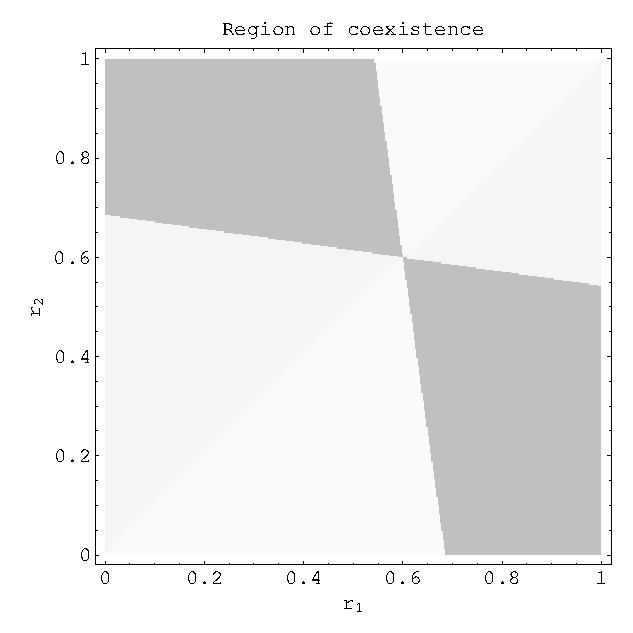
\includegraphics[scale=0.4]{figures/fig4rc}
		% 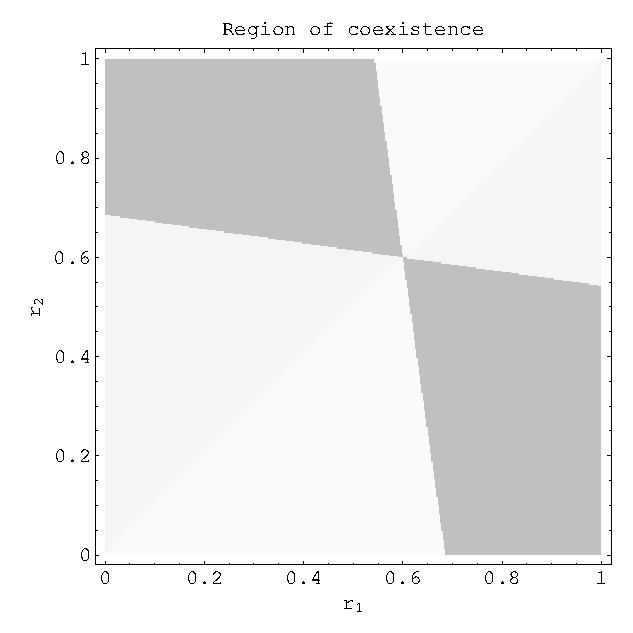
\includegraphics[scale=0.4]{figures/fig4rc}
	\end{tabular}
	\caption{Illustration of the graphical method for obtaining the region of coexistence. a) 
	A pairwise invasibility plot from the Snowdrift game \citep{Doebeli:2004}. b) The same pairwise invasibility plot mirrored over the 
	main diagonal. c) The first two panels overlaid in which the region of coexistence is 
	visible as the dark grey area. Note that protected dimorphisms are possible even though 
	the singular strategy is evolutionarily stable and selection thus stabilising. }
\label{coexistence}
\end{figure}

\subsection{Invasion exponent and selection gradients in polymorphic populations}

The invasion exponent is generalised to dimorphic populations in a
straightforward manner, as the expected growth rate $S_{r_1, r_2}(m)$
of a rare mutant in the environment set by the two morphs $r_1$ and
$r_2$. The slope of the local fitness landscape for a mutant close to
$r_1$ or $r_2$ is now given by the selection gradients
%
$$S_{r_1, r_2}'(r_1) \,\,\, \textrm{ and } \,\,\, S_{r_1, r_2}'(r_2).$$
%
In practise, it is often difficult to determine the dimorphic
selection gradient and invasion exponent analytically, and one often
has to resort to numerical computations.

\subsection{Evolutionary branching} \label{polybranch}

The emergence of protected dimorphism near singular points during the
course of evolution is not unusual, but its significance depends on
whether selection is stabilising or disruptive. In the latter case,
the traits of the two morphs will diverge in a process often referred to 
as evolutionary branching. \citet{Geritz:1998} presents a compelling
argument that disruptive selection only occurs near fitness minima. To
understand this heuristically consider a dimorphic population $r_1$
and $r_2$ near a singular point. By continuity $S_r(m) \approx S_{r_1,
r_2}(m)$ and, since $S_{r_1, r_2}(r_1) = S_{r_1, r_2}(r_2) = 0$, the
fitness landscape for the dimorphic population must be a perturbation
of that shown in Figure \ref{SinS}a with the region of positive
invasion fitness lying between $r_1$ and $r_2$.

\subsection{Trait evolution plots}

Evolution after branching is illustrated using trait evolution
plots. These show the region of coexistence, the direction of
evolutionary change and whether points where points where the
selection gradient vanishes are fitness maxima or minima. Evolution
may well lead the dimorphic population outside the region of
coexistence, in which case one morph is extinct and the population
once again becomes monomorphic.

\begin{figure}
\begin{tabular}{ll}
	 \includegraphics[width=0.49\textwidth]{figures/polyPIP} &
	 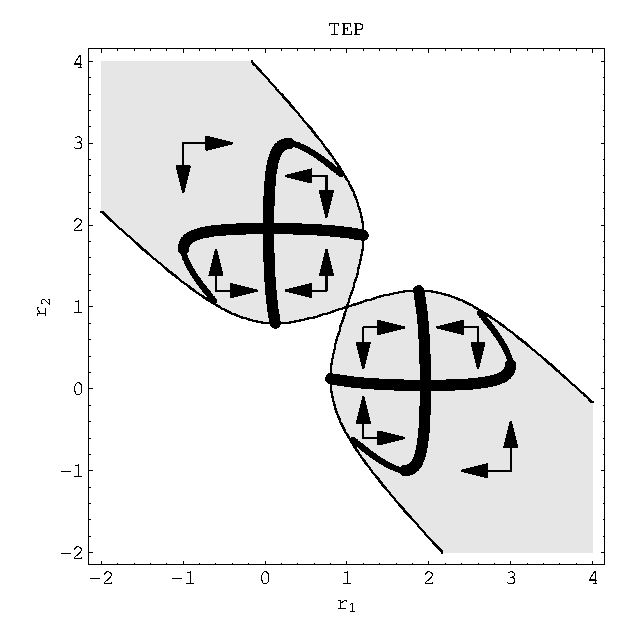
\includegraphics[width=0.49\textwidth]{figures/polyTEP} 
\end{tabular}
\caption{Levene's soft selection model studied by
\citet{Geritz:1998}. The pairwise invasibility plot shows the
evolutionary dynamics for a monomorphic population. Since selection at
the convergence stable singular point is disruptive, the population
eventually becomes dimorphic with evolutionary dynamics given by the
trait evolution plot. The arrows show the direction of
evolutionary change. Thick lines are evolutionarily stable isoclines,
where directional selection in one of the two morphs cease. In this 
case, the trait evolution plot shows the final evolutionary outcome
to be a stable protected dimorphisms with approximate trait values 
$r_1 = 2$ and $r_2 = 0$ where the ordering is arbitrary.}
\label{mip}
\end{figure}

Figure \ref{mip} shows an example of a trait evolution plot. The
lines are \emph{evolutionary isoclines} where one of the two selection
gradients vanishes. These are found by solving 
%
$$S_{r_1, r_2}'(r_1) = 0 \,\,\, \textrm{ or } \,\,\, S_{r_1, r_2}'(r_2) = 0.$$
%
An isocline can be either a fitness maximum or fitness minima for
mutants close to the morph (in fact the situation is exactly identical
to the monomorphic case if we consider the other morph as being a
constant part of the environment). We recommend using the same
conventions as \citet{Geritz:1998}, that is using thin lines to denote
fitness minima, and thick lines for fitness maxima.

\subsection{Evolutionarily singular coalitions}

An intersections of two isoclines at a point is known as a singular
coalitions \citet{Geritz:1998}. If the strategies $r_1$ and $r_2$ at
the intersection are stable strategies when considered separately with
the other trait value fixed the coalition is stable and represent a
possible endpoint where evolutionary change cease. To test for
stability the analytical condition for evolutionary stability can be
applied to each morph, however there is no natural generalisation of a
CSS \citep{Geritz:1998} and convergence stability is most easily
inferred directly from the trait evolution plot.

\subsection{Connection of the isoclines to the boundary}

The boundaries of the region of coexistence are extinction threshold for
morphs, and hence for a dimorphic population $r_1$ and $r_2$ the
boundary where $r_2$ becomes extinct is given implicitly by
$S_{r_1}(r_2) = 1$ and for points in the region of coexistence close
to this boundary the approximate relationship $S_{r_1, r_2}(m) \approx
S_{r_1}(m)$ holds.  This simple observation has implications for the
connection of the isoclines to the boundary. If $S'_{r_1, r_2}(r_1) =
0$ on the boundary we also have $S_{r_1}'(r_1)=0$ so $r_1$ must be a
singular point of a monomorphic population. 

The isoclines defined by $S'_{r_1, r_2}(r_2) = 0$ connects to the
boundary where it has a vertical tangent. The reason is that at every
other point on the boundary, the selection gradient for $r_2$ points
towards the interior of the region of coexistence (either up or
down). If the isocline would connected to such a point it would divide
the region into two areas where the selection gradient for $r_2$
points in opposing directions, and one of these would not be towards
the interior which is a contradiction. By symmetry we get
corresponding results for the other isoclines. For a more detailed
discussion see \citet{Geritz:1998}

\subsection{Further evolutionary branching}

Evolutionary branching in a morph $r_1$ under small but fixed
mutational steps may occur whenever the fitness landscape as given by
the function $S_{r_1, r_2}(m)$ has a local minimum at $r_1$. The most
likely branching point is an unstable singular coalition, but branching could
also happen along an isocline.


\section{Example}

% Enkel birth-death process.
% Samma men med ESS

% Branching in host-parasite system. 
% Spelteori?

To clarify the basic concepts for monomorphic populations we now
consider a population of $n$ individuals where individuals reproduce
at a rate $b$ and die with the density-dependent rate $dn$. The number
of individuals $n(t)$ at time $t$ then grows logistically according to
the linear differential equation $n'(t) = n(t)(b - n(t)d)$ subject to
some initial condition $n(0)=n_0$.  In particular the equilibrium
population density $n^*$ is found by solving $0 = n^*(b - dn^*)$ with
the non-trivial solution $n^* = b/d$. Though not relevant here, it
should be noted that a change of time-scale reduces the number of
parameters to 1.

We will now assume that the birth-rate is subject to evolutionary
change without constraint. The model must now be extended to include, at
the very minimum, two populations $n_1$ and $n_2$ with respective
trait values $b_1$ and $b_2$. Writing $n(t) = n_1(t) + n_2(t)$ we have
%
\begin{equation} \label{example_system}
	n'(t) = b_1 n_1(t) + b_2 n_2(t) - d n(t)^2
\end{equation}	
%
We now introduce the suggestive notation $n_r(t) = n_1(t)$, $r = b_1$
and $n_m(t) = n_2(t)$, $m = b_2$ for the respective trait values of
the resident and mutant type. The invasion exponent is then
defined as the initial per-capita growth rate of the mutant when it
enters the equilibrium environment set by the mutant, which in this
situation amounts to the logarithmic derivative of $n_2$ evaluated 
for $n_r = n^*$ and $n_m = 0$
%
$$S_r(m) = m - r.$$
%
\begin{figure}
	\begin{tabular}{ll}
		\includegraphics[width=0.49\textwidth]{figures/examplePIP1} &
		\includegraphics[width=0.49\textwidth]{figures/examplePIP2}
	\end{tabular}
	\caption{Pairwise invasibility plots of the example of a birth-death system. The relevant trait 
	is the birth rate here. 
	a) PIP according to the system given in (\ref{example_system}). The birth rate can evolve 
	to ever higher values.  b) PIP according 
	to the system given in \ref{example_system2} with $c(r) = 10^{-1} \exp(r)$. The singular point is evolutionarily 
	and convergence stable and located at $r \approx 2.3.$}
\label{example1}
\end{figure}
Note that in particular $S_r(r)$ = 0. The corresponding pair-wise
invasibility plot is given in Figure \ref{example1}a. As expected, the
birth rate evolves towards ever higher values. We can change this by
introducing a cost of higher birth rates 
%
\begin{equation} \label{example_system2}
n'(t) = n(t)(r - c(r) - n(t)d)
\end{equation}
yielding the invasion exponent 
%
$$S_r(m) = m - c(m) - r + c(r).  $$
%
Provided $b-c(b)$ is bounded we expect an evolutionary endpoint as a
convergence and evolutionarily stable strategy according to criteria
(\ref{ESScriterion}) and (\ref{CSScriterion}). For $c(r) = 10^{-1}
\exp(r)$ we get the pairwise invasibility plot shown in Figure
\ref{example1}b with the singular point at $r=\ln(10)\approx 2.3$.

\section{Discussion}

The aim of this manuscript has been to introduce the basic concepts of
Adaptive Dynamics. As with any introductory text, there are many
issues that we have not touched upon. These include aspects of the treatment 
of higher dimensional traits, the problem of finding conditions for when a
successfully invading mutant successfully ousts the resident, and the
possibility of incorporating genetic detail. We have also left out any
discussion of the implications of evolutionary branching--one of the
most interesting findings of Adaptive Dynamics--for understanding
speciation in sexually reproducing populations.

Even though there are many areas of Adaptive Dynamics which we haven't
covered, the basic techniques are usually sufficient for practical
purposes, and when not the material in this manuscript should be
enough to read and understand many of the articles that advances or
uses the theory.

\section{Further reading} \label{further_reading}

A good introductory text to Adaptive Dynamics is
\citet{Diekmann:2003}, which presents the basics of monomorphic
evolution using many instructive examples. The next natural step is
\citet{Geritz:1998} and \citet{Metz:1996} which describe the theory
in depth. To better understand how the techniques can be used in
studying more complex models, a manuscript studying a sample model
such as \citet{Geritz:1999} or \citet{Brannstrom:2005b} may prove
helpful.

The canonical equation is introduced by \citet{Dieckmann:1996},
studied in more detail by \citet{Champagnat:2001} and extended to
physiologically structured populations in \citet{Durinx:2005}.
\citet{Champagnat:2006} puts this into context by considering ways
in which microscopic stochastic processes can be studied on a
macroscopic scale. \citet{Geritz:2002} introduces the \emph{Tube
Theorem} which says that the sum of the resident and a sufficiently
similar mutant populations canonically remain inside a `tube'. Two
more recent publications about the population dynamical
foundations, basically the study of when a successfully invading
mutant may be expected to replace the resident population, are
\citet{Geritz:2003} and \citet{Gyllenberg:2003}.  This is an active
area of research, so please check the forward citations for the latest
developments.
 
A list of articles related to Adaptive Dynamics is currently
maintained by \'Eva Kisdi at
\verb+http://www.helsinki.fi/~mgyllenb/addyn.htm+. For an
enjoyable evening read in front of the fireplace we recommend
\citet{Leimar:2001} which argues that a `Darwinian demon' able to
control the mutations that occur can have a profound impact on
evolution even if the actual population dynamics is beyond its
control.


\section{Acknowledgements}
We thank Hans Metz and Jacob Johansson for valuable comments and
suggestions and Bernd Blasius and Thilo Gross from the University of
Potsdam for inviting us to the Stanislaw Lem workshop on evolution in
Lviv, Ukrainia. \AA{}.B. gratefully acknowledges support from the
Japan Society for the Promotion of Science, and would like to thank
Ulf Dieckmann, Hans Metz, Karl Sigmund and Fugo Takasu for many useful
discussions about Adaptive Dynamics and its applications.

\section{About this document}

The latest version of this document is kept at
\verb+http://adtoolkit.sourceforge.net+, together with a free
Mathematica package for generating pairwise and trait evolution
plot. Permission is granted to copy, distribute and/or modify this
document under the terms of the GNU Free Documentation License,
Version 1.2 or any later version published by the Free Software
Foundation; with no Invariant Sections, no Front-Cover Texts, and no
Back-Cover Texts.

\appendix

\section{Appendix}

\subsection{Local classification of singular points} \label{classification}

For a mathematical derivation of the criteria of ESS, CSS, and dimorphism we first need to conceive the invasion exponent $S_r(m)$ depending on $m$ with the
coefficient $r$ as a function depending on two variables: $S_r(m) \equiv S(r,m)$. Both perspectives are exactly equivalent, but with the invasion
exponent $S$ seen as a map representing a two-dimensional fitness landscape as in the PIPs in
Fig. \ref{PIPs} heuristic analytical arguments can easily be used for classification.
We focus on the curvature of $S(r,m)$ landscape at singular points given in the second order derivatives
following the argumentation of \citet{Geritz:1998}.
The ESS criterion doesn't depend on the curvature in the direction of changed resident traits $r$ and simply
corresponds to the condition for a local maximum as argued in section \ref{EsinS}
%
$$
   \frac{\partial^2 S}{ \partial m^2} \Big| _{r=m=r^*} < 0 \quad (\mathrm{ESS \ criterion}).
$$
%
For a singular strategy to be CSS the selection gradient needs to point towards the singular strategy, i.e.
its sign changes from positive to negative when going through $r^*$. So $S'_r(m)$ must be a decreasing function
near the singular point

\begin{equation} \label{someq}
   \frac{d}{dr} S'_{r}(r) = \frac{\partial^2 S}{ \partial r^2} \Big| _{r=m=r^*}+  \frac{\partial^2 S}{ \partial m \partial r}\Big| _{r=m=r^*}  < 0.
\end{equation}

Since $S_r(r) = 0$ we have

\begin{equation} \label{bigtrick}
0 = \left(\frac{d}{dr}\right)^2 S_r(r) = \frac{\partial^2 S}{ \partial r^2} \Big| _{m=r} +  2\frac{\partial^2 S}{ \partial m \partial r}\Big| _{m=r} +\frac{\partial^2 S}{ \partial m^2}\Big| _{m=r}
\end{equation}

and thus (\ref{someq}) can be  rewritten as

\begin{equation} \label{CSSfinally}    
	\frac{\partial^2 S}{ \partial r^2} \Big| _{r=m=r^*} >  \frac{\partial^2  S}{\partial^2 m}\Big| _{r=m=r^*} \quad (\mathrm{CSS \ criterion}).
\end{equation}

If a singular point is convergence stable but evolutionarily unstable,
selection near the singular point is disruptive and evolutionary
branching will eventually occur. However, even with stabilising
selection protected dimorphism may occur near a singular point
provided there are points near the singular strategy where both
$S(r,m)$ and $S(m,r)$ are positive. This means that the line $m =
2r^*- r$ passing through the singular point at an angle of -45� must
locally be in a region where $S$ is positive. Thus, $S(r,2r^*- r)$
must have a minimum at $r^*$ meaning that at this point its second
derivative is positive. Hence,
%
$$
   \frac{\partial^2  S}{ \partial m^2}\Big| _{r=m=r^*}- 2 \frac{\partial^2 S}{\partial r \partial m}\Big| _{r=m=r^*} + \frac{\partial^2 S}{\partial r^2}\Big| _{r=m=r^*} > 0.
$$
%
which using again (\ref{bigtrick}) gives the criterion
%
$$
   \frac{\partial^2 S}{ \partial m^2}\Big| _{r=m=r^*} >  -\frac{\partial^2 S}{\partial r^2}\Big| _{r=m=r^*} \quad (\mathrm{dimorphism \ criterion})
$$
%
for protected dimorphisms to exist near the singular strategy.


\subsection{Terms and concepts in brief}

\begin{tabular}{|p{0.4\textwidth}p{0.6\textwidth}|}
\hline
\textbf{Term} & \textbf{Description} \\
\hline
&\\
\textit{invasion exponent} & Function giving the expected growth rate of a rare mutant \\
%
\textit{selection gradient} & Derivative of the invasion exponent with respect to the mutant trait evaluated at the resident trait value. Gives information on 
the direction and speed of evolutionary change.  \\
%
\textit{Evolutionarily singular strategy} & Point or strategy where the selection gradient vanishes.\\ 
\textit{Evolutionarily stable strategy} & Singular strategy that cannot be invaded by (locally) neighbouring mutants. \\ 
\textit{Convergence stable strategy} & Singular strategy which, within a neighbourhood, is approached gradually.\\ 
\textit{Monomorphic population} & Population consisting of only one phenotype. \\
\textit{Dimorphic population} & Population with two phenotypes. \\
\textit{Polymorphic population} & Population with several phenotypes. \\
\textit{Pairwise invasibility plot} & Graphical illustration of invasion success for monomorphic populations. \\
\textit{Trait evolution plots} & Graphical illustration of invasion success when 
	the population is dimorphic. \\
\textit{Canonical equation} & Differential equation describing a deterministic approximation of evolutionary dynamics with small mutational steps. \\
\hline
\end{tabular}

\bibliographystyle{natbib}
\bibliography{referenser}

\end{document}
